%!TEX root = ../dissertation.tex
\begin{savequote}[75mm]
There are some things you learn best in calm, and some in storm.
\qauthor{Willa Cather}
\end{savequote}

\chapter{Apache Storm}

Apache Storm is a reliable, distributed and fault-tolerant system for stream processing.
The beginnings of the project were at Backtype (later bought by Twitter) and created by Nathan Marz.
He open sourced Storm on September the 19th in 2011. The project rapidly got a big development coummunity and
on September the 18, 2013 Nathan moved Storme to Apache Incubator.\\

Storm works with different types of components which are responsible for clear defined task.
This components are bundled and managed in a so called \textbf{Topology}.
The entrypoint and the stream input is handled by a \textbf{Spout}, the spout passes to \textbf{Bolts}.
Bolts are responsible for the main data processing and persists the data.
They can be chained or parallelised in a way that fits best for your current problem.

\begin{figure}[hp]
\centering
\captionsetup{justification=centering}
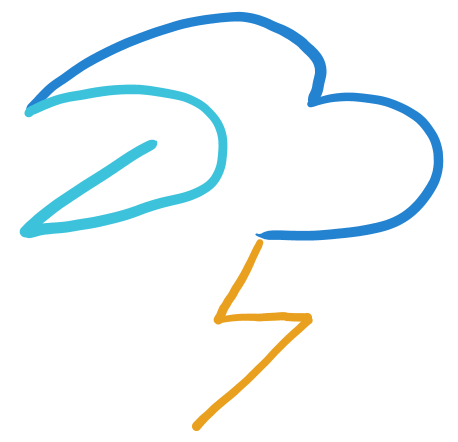
\includegraphics[width=100pt]{images/storm.png}
\caption[Storm]{Storm}
\end{figure}

\newpage

\section{Topology}
In generell Storm passes tuples between the different components.
To organize this tuples there are topologies.

\subsection{Grouping}
The Topology defines the grouping, this means how streams are consumed by the bolts and how they consume them.
There are four kinds of grouping \textit{Shuffle Grouping}, \textit{Fields Grouping},
\textit{All Grouping} and \textit{Custom Grouping}.

\subsubsection{Shuffle Grouping}
Shuffle Grouping takes a single entry from the source and sends each tuple to a randomly choosen bolt,
which is listening to this kind of tuples. It also garanties that each consumer get's the same number of tuples.

\subsubsection{Fields Grouping}
With Fields Grouping it is possible to send toples to spezified bolts based on the fields of the tuple.
It takes care that the same combination of fields is always sent to the same bolt.

\subsubsection{All Grouping}
All Grouping sends every tuple to all the bolts. This is helpful for tasks like signals or
use different filters for alerting systems.

\subsubsection{Custom Grouping}
It is possible to build your on grouping based on the stream. This is very helpful if you have to make
fine granular desicions about which bolt has to handle which tuple.


\newpage

\section{Spout}
The entry point of each topology are the so called spouts. The spouts are responsible for their reliability,
thus you have to take care to implement them in a fault-tolerant way. This means that a spout must have the
ability to deal with unprocessable messages from the stream.\\
To handle the reliability at the spout you can add an ID to every message. If a message is correctly processed  by
all the target bolts the \textit{ack} method of the spout is called. But if there were troubles or the timeout is
reached the \textit{fail} method will be triggered.

\newpage

\section{Bolt}

